\documentclass[zh]{thesis}  % draft mode (default)
%\documentclass[review]{thesis}  % review mode (show contents & reference only)
%\documentclass[watermark,final]{thesis}  % final mode (version for library)

%-------------------------------------------------------------------------------
% Package Loading
%-------------------------------------------------------------------------------

\usepackage{multirow}     % for multi-row table
\usepackage{booktabs}     % table style used in books
\usepackage{cite}
\usepackage{pdfpages}     % input pdf
\usepackage{amsmath,amsthm,amssymb}
\usepackage{fontspec}
\usepackage{xcolor}
\usepackage{colortbl,booktabs}
\usepackage{titlesec}
%\usepackage{bbding}
%-------------------------------------------------------------------------------
% Configuration
%-------------------------------------------------------------------------------

% 填寫題目, 作者, 指導教授, 學校, 系所, 日期等資訊
% Title
\title{Analyzing Product Semantic Labels as Cue for placing action - Product Semantic dataset and Cooperative Dual-Arm Active Manipulation}
\titlezh{分析商品語意作為擺放行為之線索 – 商品語意資料集建置與雙手臂主動式操作}

% Author
\author{Yung-Shan Su}
\authorzh{蘇詠善}

% Advisor
\advisor{Hsueh-Cheng Wang}
\advisorzh{王學誠}

% First co-advisor (Leave {} empty if you don't have a co-advisor)
\coadvisoA{}
\coadvisorAzh{}

% Second co-advisor (Leave {} empty if you don't have a second co-advisor)
\coadvisorB{}
\coadvisorBzh{}

% Field
\field{Electrical Engineering}

% Institute
\institute{Institute of Electrical Control Engineering}
\institutezh{電控工程研究所}

% College
\college{College of Electrical and Computer Engineering}

% University
\university{National Chiao Tung University}
\universityzh{國立交通大學}

% Location
\location{Hsinchu, Taiwan}

% Date of final submission
\degreemonth{March}
\degreeyear{2019}
\degreeyearzh{中 華 民 國 一 百 零 八 年 三 月}

% Watermark
\watermark{figures/nctu_logo.jpg}


% 修改 thesis.cls 的預設字型
%-------------------------------------------------------------------------------
% Chinese Font Settings
%
%   These macros are used to change the default Chinese fonts (see below) used
% by thesis.cls. Please leave {} empty if you want to use the default settings
% and make sure that you have added '-shell-escape' option when using xetex to
% compile tex files, i.e. xetex compiling commands should run something like:
%
%     xelatex -synctex=1 -shell-escape -interaction=nonstopmode %.tex
%
% (default Chinese font settings)
%   Windows              Linux                        Mac OS X
% * 標楷體 (DFKai-SB)    AR PL 中楷 (AR PL UKai TW)   楷體-繁 (Kaiti TC Regular)
% @ 新細明體 (PMingLiU)  AR PL 明體 (AR PL UMing TW)  儷宋 Pro (LiSong Pro)
%
% * fontname --> 預設中文本文字型 (serif)
% @ fontname --> 預設中文明體字型 (sans-serif, 使用於封面頁)
%-------------------------------------------------------------------------------

% main (serif) Chinese font, leave {} empty to enable default font setting
\mainfontzh{}

% sans-serif Chinese font, leave {} empty to enable default font setting
\sansfontzh{}

%-------------------------------------------------------------------------------
% English Font Settings
%
%   These macros are used to change the default English fonts (see below) used
% by thesis.cls. Please leave {} empty if you want to use the default settings.
%
% (default English font settings)
% main font       --> Times New Roman (for all platforms)
% sans-serif font --> Arial           (for all platforms)
%-------------------------------------------------------------------------------

% main font for English, leave {} empty if you want to use default font setting
\mainfont{}

% sans-serif font for English, leave {} empty if you want to use default setting
\sansfont{}



\begin{document}

% Show repeated author names in bibliography when using IEEEtran.bst
% Comment out this line if you don't set IEEEtran in \bibliographystyle{}
\bstctlcite{IEEEexample:BSTcontrol}

% Generate cover, title, authorization, approval and copyright pages
\maketitle

%-------------------------------------------------------------------------------
% Abstract
%-------------------------------------------------------------------------------

% 中文摘要
\begin{abstractzh}

在人類只喝酒和茶的時候時候, 文明是健全的. 當開始喝起咖啡或可樂這些泥水色的飲料後,就開始了頹廢和墮落.

\end{abstractzh}

% 英文摘要
\begin{abstract}%

The humanity falls when people start to drink coffee and coke ...

\end{abstract}

%-------------------------------------------------------------------------------
% Acknowledgement
%-------------------------------------------------------------------------------

% 誌謝
\begin{acknowledgement}

Thanks to my wife, Frederica Greenhill, who makes delicious sandwiches for me always.

\end{acknowledgement}

% 題獻頁 (Only shown in the final mode of a PhD dissertation)
%\begin{dedication}%

\textit{Dedicated to RTES Lab $@$ NCTU}\\

{\Large 為了健康和美容, 飯後要喝一杯紅茶.}\\

\end{dedication}

%-------------------------------------------------------------------------------
% 目錄
%-------------------------------------------------------------------------------

% Generate 'Table of Contents', 'List of Figures', and 'List of Tables', and
% Set page numbering to 'arabic'
\maketocs

%-------------------------------------------------------------------------------
% Contents
%-------------------------------------------------------------------------------

% Set page numbering to 'arabic' (1, 2, 3, ...)
\mainmatter

% 內文, 請依照章節順序擺放
\chapter{緒論}
\label{chapter:intro}

\section{背景與動機}

在人工智慧的浪潮下, 已有愈來愈多工廠只餘機器人在工作, 人們只需定期去工廠檢
查確保正常營運。科技技術的進步往往能便利人們的生活,也漸漸改變人們生活的方
式, 以日常生活舉例, 當需要購買生活用品時會去便利超商、量販店或是直接由網路購
物商城購買商品, 最近更出現了不須服務人員的無人商店, 如: 位於西雅圖的 AmazonGo
無人商店, 主打顧客挑選商品完就可以帶著商品離開, 不須交由店員結帳付款, 而是自動
辨識顧客挑選的商品進行信用卡扣款, 省去了等待排隊的時間; 而網路購物也是相當便
利, 由廠商針對顧客網路訂單從倉儲進行集貨並由貨運公司進行運輸到客戶手中,其中
許多廠商為了提高集貨的效率已經著手於倉儲的自動化。然而在無人商店跟倉庫的應
用中,現今還無法達成實質無人化,原因是因為如無人商店內商品上架仍需人去逐一
整齊擺放,而倉庫在進行商品分類與打包時也須有人去掃描商品條碼才可以知道商品
代號和該怎麼打包。這些自動化任務成了現在業界都想解決的問題。


而亞馬遜揀取挑戰Amazon Picking Challenge,便因此而生。在自動化的亞馬遜公司倉庫中,成千上萬的移動機器人將1平方公尺的貨架單元從存儲位置移動到揀選區,然後再移回存儲位置。工人須站在揀選區,從貨架上挑選物品,並將它們放入運往客戶的箱子中。貨架上的典型箱中最多可包含10個物品 - 通常緊密堆積在一起 , 員工可以識別正確的產品,從箱子中取出,掃描條形碼進行驗證,然後放置物品在一個盒子裡,所有這些都只需幾秒鐘。典型的亞馬遜倉庫擁有數百萬種不同的產品。雖然許多這些物品形狀簡單,如書籍和DVD,但也有如泰迪熊,兒童項鍊,真空包裝的USB棒,這些不規則的其他形狀、物品。在這過程中目前仍無法省略的便是人工揀取物品放置箱子的流程。因此亞馬遜公司認為自動化揀取是機器人操作中一個相當重要的技術,並且將可應用於許多領域上如倉庫、大量製作、服務機器人(service robotics)上。為了自動化這個任務,亞馬遜公司連續3年舉辦亞馬遜揀取競賽,並祭出高額獎金,邀請機器人名校來解決自動化夾取問題。由此可知自動化夾取問題的重要性。


然而除了自動化夾取任務外,放置也是相當重要的議題,如上述所提無人商店上架,除了將商品揀取放上架子外,還要確保架上的商品是否有擺正,也就是商品商標或是品牌文字是否有朝外。而在倉庫中生產線分類物品時,也須將物品夾取並放置到輸送帶上,並確保條型碼朝上,以便掃描機能掃描條碼進行分類。這兩者任務雖有所不同,但皆可歸類為需針對商品上語意標籤如品牌文字或條碼去進行套定姿態擺放任務。結合語意標籤進行特定姿勢擺放任務是一
較新穎之領域, 相當具有挑戰性。便可實際應用於倉庫與無人商店,將可降低大量人力
與時間成本。


\section{目標與貢獻}

\subsection{問題定義}
在無人商店與倉庫的許多應用中,夾取與放置任務都十分重要,如無人商店上架必
須放置商品時,品牌文字或商標需朝外放。放置任務尤其以特定姿態放置任務最為困
難,因為其牽涉到物品姿態以及夾取可行性。在此研究中,我將物品表面的一小部分
作為語意標籤, 此語意標籤不僅可以作為物品三維姿態辨識的依據, 更可以做為操作行
為的依據, 物品上可能有不只一個語意標籤如品牌文字、條形碼等, 本研究將專注於再
雜亂環境中,以品牌文字為線索進行特定姿勢放置任務。

\subsection{挑戰}
\begin{itemize}
\item 在雜亂的環境中,產品物件可能互相堆疊,造成物品部分或全部遮蔽 (occlusion)。
由於品牌文字可能只在產品物件的特定平面位置, 也可能在初始位置即被遮蔽,如何偵測品牌文字或是找出品牌文字所在的一面,是本研究重要目標之一
\item 受限於機器手臂與末端效應器(End effector)的工作範圍,即使預測出物體姿態,特定姿態夾取與放置行為仍可能無法執行,或是在移動過程中會遇到障礙物,造成任務失敗。因此夾爪的設計與實驗環境的架設,也是本研究的重要議題之一。
\end{itemize}

\subsection{論文貢獻}
\begin{itemize}
\item \textbf{主動式操作搭配雙手臂協作} 除卻被動利用物件辨識與姿態辨識的結果,本論文運用主動式操作概念去改變雜亂場景,去達到對單一物品與品牌文字最佳的的感知能力。本論文提出的方法不僅可以改變相機視角去看到最少遮蔽的品牌文字,也使用雙手臂協作的方式去操作商品,以達到最佳的放置成效。
\item \textbf{建立基準商品語意資料集以訓練與測試模型與演算法效果} 在現今的影像物件分割技術下,訓練一個深度卷積神經網路需要數量龐大且有標注的資料集。
為了訓練物件切割模型,本論文建立了一個資料集,此資料集包含20個物件,且每個物件都有條碼與品牌文字。此資料集包含來自真實世界與虛擬環境的訓練資料以及真實環境的測試集用來評估放置任務的成效。
\end{itemize}

\begin{figure}[ht]
	\centering
	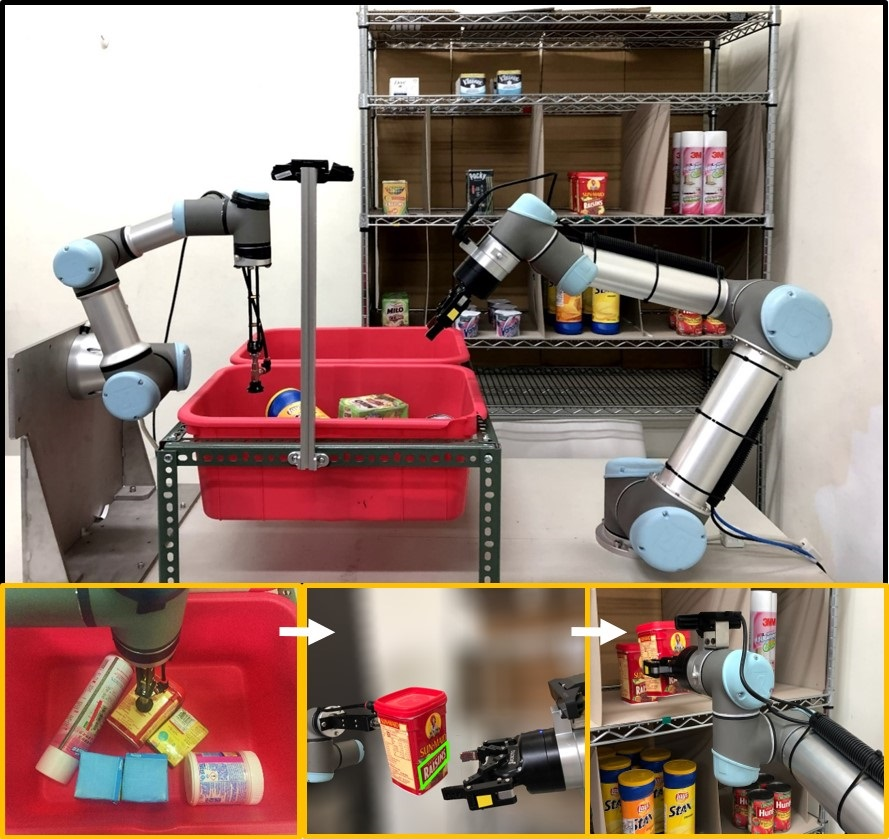
\includegraphics[height=!, width=0.7\linewidth, keepaspectratio=true]
	{./figures/pose-aware-placing-teaser-v3.jpg}
  \caption{本論文利用商品文字(商品上的其中一個語意標籤)作為特殊姿態放置的依據,並設計雙手臂協做的主動式操作系統去解決物品遮蔽的問題。圖左下到右下:吸盤式夾爪透過物品或品牌文字語意線索去夾取物品至空曠空間,而兩指式夾爪再透過品牌文字線索去執行放置任務。}
  \label{figure:teaser}
\end{figure}

\section{論文架構}
本論文架構總共有五個章節。第一章為緒論,包含背景動機、以及目標貢獻。第二章則介紹文獻回顧,包含Amazon Picking Challenge競賽回顧、主動式視覺與主動式操作系統、物品夾取可行性預測、雙手臂機械協作、機器人操作領域之基準訓練測試集,快速瀏覽在與本論文相關之研究領域,第三章則為系統架構與方法,依序介紹系統的硬體架構與工作環境、商品語意資料庫、基於品牌文字之夾取可行性預測、主動式操作系統。第四章介紹本研究的兩大實驗:品牌文字切割評估、主動式操作系統評估。最後一章為本論文的結論與未來展望。

\chapter{Related work}
\label{chapter:relate-work}

\textbf{thesis.cls} 是本 template 的核心, 其主要功能是產生論文的封面, 設定版面與章節樣式, 並提供自動選擇字型的功能.
因大部分需要使用者輸入的資訊(e.g. author name)都有拉出對應的變數讓使用者設定, 因此
絕大部分的情況下, 你是不需要動到 thesis.cls 的.
當然, 如果你有發現 bug 或是覺得哪些地方有更好的寫法, 也請麻煩在 github 上發個 issue 告訴我吧, 謝謝!

以下介紹如何設定封面資訊與字型, thesis.cls 提供的 options, 以及摘要等檔案放置的位置.

\section{封面資訊}

封面資訊的設定指令全部都放在 \textit{config/frontmatters.tex} 中, 請在此設定你論文的 title, author name, (co-)advisor name, college name (院), institute name (所), field (領域), 日期等資訊.

\textbf{注意:} 如果沒有共同指導教授, \textbackslash coadvisorA, \textbackslash coadvisorAzh, \textbackslash coadvisorB \textbackslash coadvisorBzh 的\{ \}請留白.

\section{字型設定}
\label{sec:fonts}

為了避免在不同作業系統上編譯文件時要重新設定中文字型, thesis.cls 提供了自動選擇字型的功能.
(請在 xelatex 加入 \textbf{-shell-escape} 才能開啟此功能)

\subsection{預設英文字型}

thesis.cls 預設的英文字型在全部作業系統上皆為
\begin{itemize}
\item 本文字型(main font): \textbf{Times New Roman}
\item 無襯線字型(sans-serif font): \textbf{Arial}
\end{itemize}

\subsection{預設中文字型}

thesis.cls 預設的中文字型則詳列於 Table~\ref{table:zhfonts}.
簡單來說, 本文使用``標楷體", 封面字型則使用``明體".

% table
\begin{table}[h]
\centering
% [] 顯示在 list of tables 的文字
% {} 顯示在表格上方的文字
\caption[Default Chinese font settings]{預設的中文字型}
\label{table:zhfonts}
\begin{tabular}{@{}lll@{}}
\toprule
作業系統     & 本文字型     & 明體字 (用於封面) \\ \midrule
Windows  & 標楷體      & 新細明體       \\
Linux    & AR PL 中楷 & AR PL 明體   \\
Mac OS X & 楷體-繁     & 儷宋 Pro     \\ \bottomrule
\end{tabular}
\end{table}

\subsection{修改預設字型}

thesis.cls 提供了以下四個修改預設字型的指令.
\textbf{注意: 如果修改了預設字型, thesis.cls 則不會再根據所處的作業系統自動選擇字型.}
我將此四個指令獨立出來放在 \textit{config/fonts.tex} 裡面.
如果不想修改預設字型, \{ \} 請留白.

\begin{itemize}

\item \textbf{\textbackslash mainfontzh\{\}} 修改預設中文本文字型

\item \textbf{\textbackslash mingfontzh\{\}} 修改預設中文明體字型

\item \textbf{\textbackslash mainfont\{\}} 修改預設英文本文字型

\item \textbf{\textbackslash sansfont\{\}} 修改預設英文無襯線字型

\end{itemize}


\section{Options provided by thesis.cls}

thesis.cls 提供碩士與博士論文模板, 並提供初稿與終稿等選項讓使用者自行印出的版面格式.
thesis.cls 的 options 設定就在 \textbf{main.tex} 的第一行

\textbackslash documentclass[\textbf{<options>}]\{thesis\}

以下介紹 thesis.cls 所提供的 options

\newpage

\subsection{給沒空的人看的無腦版本}

\paragraph{英文碩士論文} 請設定

\begin{itemize}
\item 初稿\\
\textbackslash documentclass[]\{thesis\}
\item 終稿\\
\textbackslash documentclass[watermark,final]\{thesis\}
\item 只顯示論文內文, 附錄, 和 reference\\
\textbackslash documentclass[review]\{thesis\}
\end{itemize}

\paragraph{中文碩士論文} 在 [ ] 中多加一個 `zh' 就會顯示中文的章節編號和標題了, 舉例來說

\begin{itemize}
\item \textbackslash documentclass[zh,watermark,final]\{thesis\}
\end{itemize}


\paragraph{英文博士論文} 請在 [ ] 中多加一個 `phd', 舉例來說

\begin{itemize}
\item \textbackslash documentclass[phd,watermark,final]\{thesis\}
\end{itemize}

\paragraph{中文博士論文} 一樣在 [ ] 中多加一個 `zh' 就可以了, 舉例來說

\begin{itemize}
\item \textbackslash documentclass[phd,zh,watermark,final]\{thesis\}
\end{itemize}

\paragraph{雙面列印} 預設為單面列印, 如果要雙面列印, 請在 [ ] 中加入 'twoside', 比方說

\begin{itemize}
\item \textbackslash documentclass[twoside,phd,watermark,final]\{thesis\}
\end{itemize}

\paragraph{Known Issue!} 在編譯過英文版後, 加入 `zh' 編譯中文版後的\textbf{第一次編譯}時, XeLaTeX 會出錯.
但只要再編譯一次就沒問題了.
也就是說從英文版轉到中文版的編譯步驟變成:

\hspace{2em} \textbf{XeLaTeX} (\textbf{\textit{Failed!}}) $\rightarrow$ \textbf{XeLaTeX} $\rightarrow$ \textbf{BibTeX} $\rightarrow$ \textbf{XeLaTeX} $\rightarrow$ \textbf{XeLaTeX}

\subsection{詳細版的 Class Options}

thesis.cls 提供的 options 詳列於 Table~\ref{table:clsoptions}.
標注 (default) 代表 thesis.cls 的預設值, 不需要寫在 [ ] 內.

% 把 table 的內容放在另一個檔案再 load, 讓 tex 看起來乾淨一點
\begin{table}[h]
\centering
% [] 顯示在 list of tables 的文字
% {} 顯示在表格上方的文字
\caption[Class options of thesis.cls]{Class options of thesis.cls}
\label{table:clsoptions}
\begin{tabular}{lll}
\toprule[1.1pt]
                      & Options   & Description\\
\midrule[1.1pt]
\multirow{2}{*}{論文類型} & master    & 碩士論文 (default)\\
                      & phd       & 博士論文\\
\midrule
\multirow{3}{*}{論文格式} & draft     & 初稿 (default)\\
                      & final     & 終稿\\
                      & review    & 只顯示內文,參考文獻,與附錄\\
\midrule
\multirow{2}{*}{語言}   & en        & 英文章節編號與標題 (default)\\
                       & zh        & 中文章節編號與標題\\
\midrule
\multirow{2}{*}{列印}   & oneside   & 單面列印 (default)\\

                        & twoside   & 雙面列印\\
\midrule
浮水印                   & watermark & \begin{tabular}[c]{@{}l@{}}review mode 不顯示\\ draft mode 顯示 ``DRAFT" 字樣\\ final mode 顯示指定的浮水印\end{tabular} \\
\midrule
裝訂                    & binding   & \begin{tabular}[c]{@{}l@{}} 在 final mode 預設為開啟, 保留 1cm 的裝訂空間\\ 在 review 和 draft mode 將文章置中不保留裝訂空間\end{tabular}\\
\bottomrule[1.1pt]
\end{tabular}
\end{table}


\section{論文檔案位置}

Table~\ref{table:pages} 詳列了摘要, 誌謝等頁面的位置.
如果你使用 Texmaker 之類的 editor 的話, 可以從 main.tex 連結到這些檔案.

\textbf{注意:} 題獻頁, 自傳, 著作目錄只有博士論文才需要填寫, 也只有在 \textbackslash documentclass[] 加入 `phd' 選項後才會被編譯.

\begin{table}[h]
\centering
% [] 顯示在 list of tables 的文字
% {} 顯示在表格上方的文字
\caption[檔案位置]{檔案位置}
\label{table:pages}
\begin{tabular}{@{}ll@{}}
\toprule
     & 位置                      \\ \midrule
中文摘要 & abs/abstract\_zh.tex    \\
英文摘要 & abs/abstract\_en.tex    \\
誌謝   & ack/ack.tex             \\
題獻頁  & ack/dedication.tex      \\
自傳   & author/cv.tex           \\
著作目錄 & author/publications.tex \\ \bottomrule
\end{tabular}
\end{table}

至於論文內文的檔案要放哪裡, 則看個人喜好.
我自己的習慣是把論文的每一個 chapter 獨立成一個 .tex 檔, 放在 \textit{chapters/} 下.
而附錄也是寫成獨立的 .tex 檔, 放在另一個資料夾下, 方便管理.
請參考此 template 的 \textit{chapters/} 與 \textit{appx/} 兩個資料夾.

\chapter{系統架構與方法}
\label{chapter:system}



\section{系統架構}
\label{sec:systemarchi}
本研究專注於透過設計資料庫並用其資料訓練夾取可行性預測系統,並以此作為線索作為雙手臂主動式操作系統的策略因此可分為三大部分:商品語意基準資料庫、夾取可行性預測系統、雙手臂主動式操作系統。基準資料庫目的在設計一個專門給日常商品的資料庫,此資料庫包含物品場景圖片、商品語意如商品整體遮罩、條碼遮罩、品牌文字遮罩,因此可利用這份資料集訓練夾取可行性預測系統,基準資料庫包含參考Amazon Picking Challenge來選取物品、實驗環境設計、並分別搭建現實與虛擬環境以蒐集資料並加以驗證。而夾取可行性預測系統則是改善~\cite{peterthesis}所提出之商品文字姿態估計系統之缺點,並改良成雙手臂夾取可行性預測系統,此系統包含品牌文字、物品語意分割、以及基於語意與三維點雲資訊之夾取可行性預測。而最後的雙手臂主動式操作系統則是設計雙手臂協作方式、手臂功能、假爪選擇與設計、以及最後執行任務之有限狀態機(Finite State Machine)。此系統的設計考量與基準資料庫物品選擇、夾取可行性預測系統環環相扣,因此接下來將先說明環境架設以及主動式操作系統硬體設計,接下來依序說明如何蒐集商品語意基準資料庫、夾取可行性預測系統。最後以主動式操作系統有限狀態機總結整體系統。

\section{硬體架構}
本研究專注於透過設計資料庫並用其資料訓練夾取可行性預測系統,並以此作為線索作為雙手臂主動式操

\begin{figure*}[htb]
   \centering
     \begin{subfigure}[t] {0.43\textwidth}
          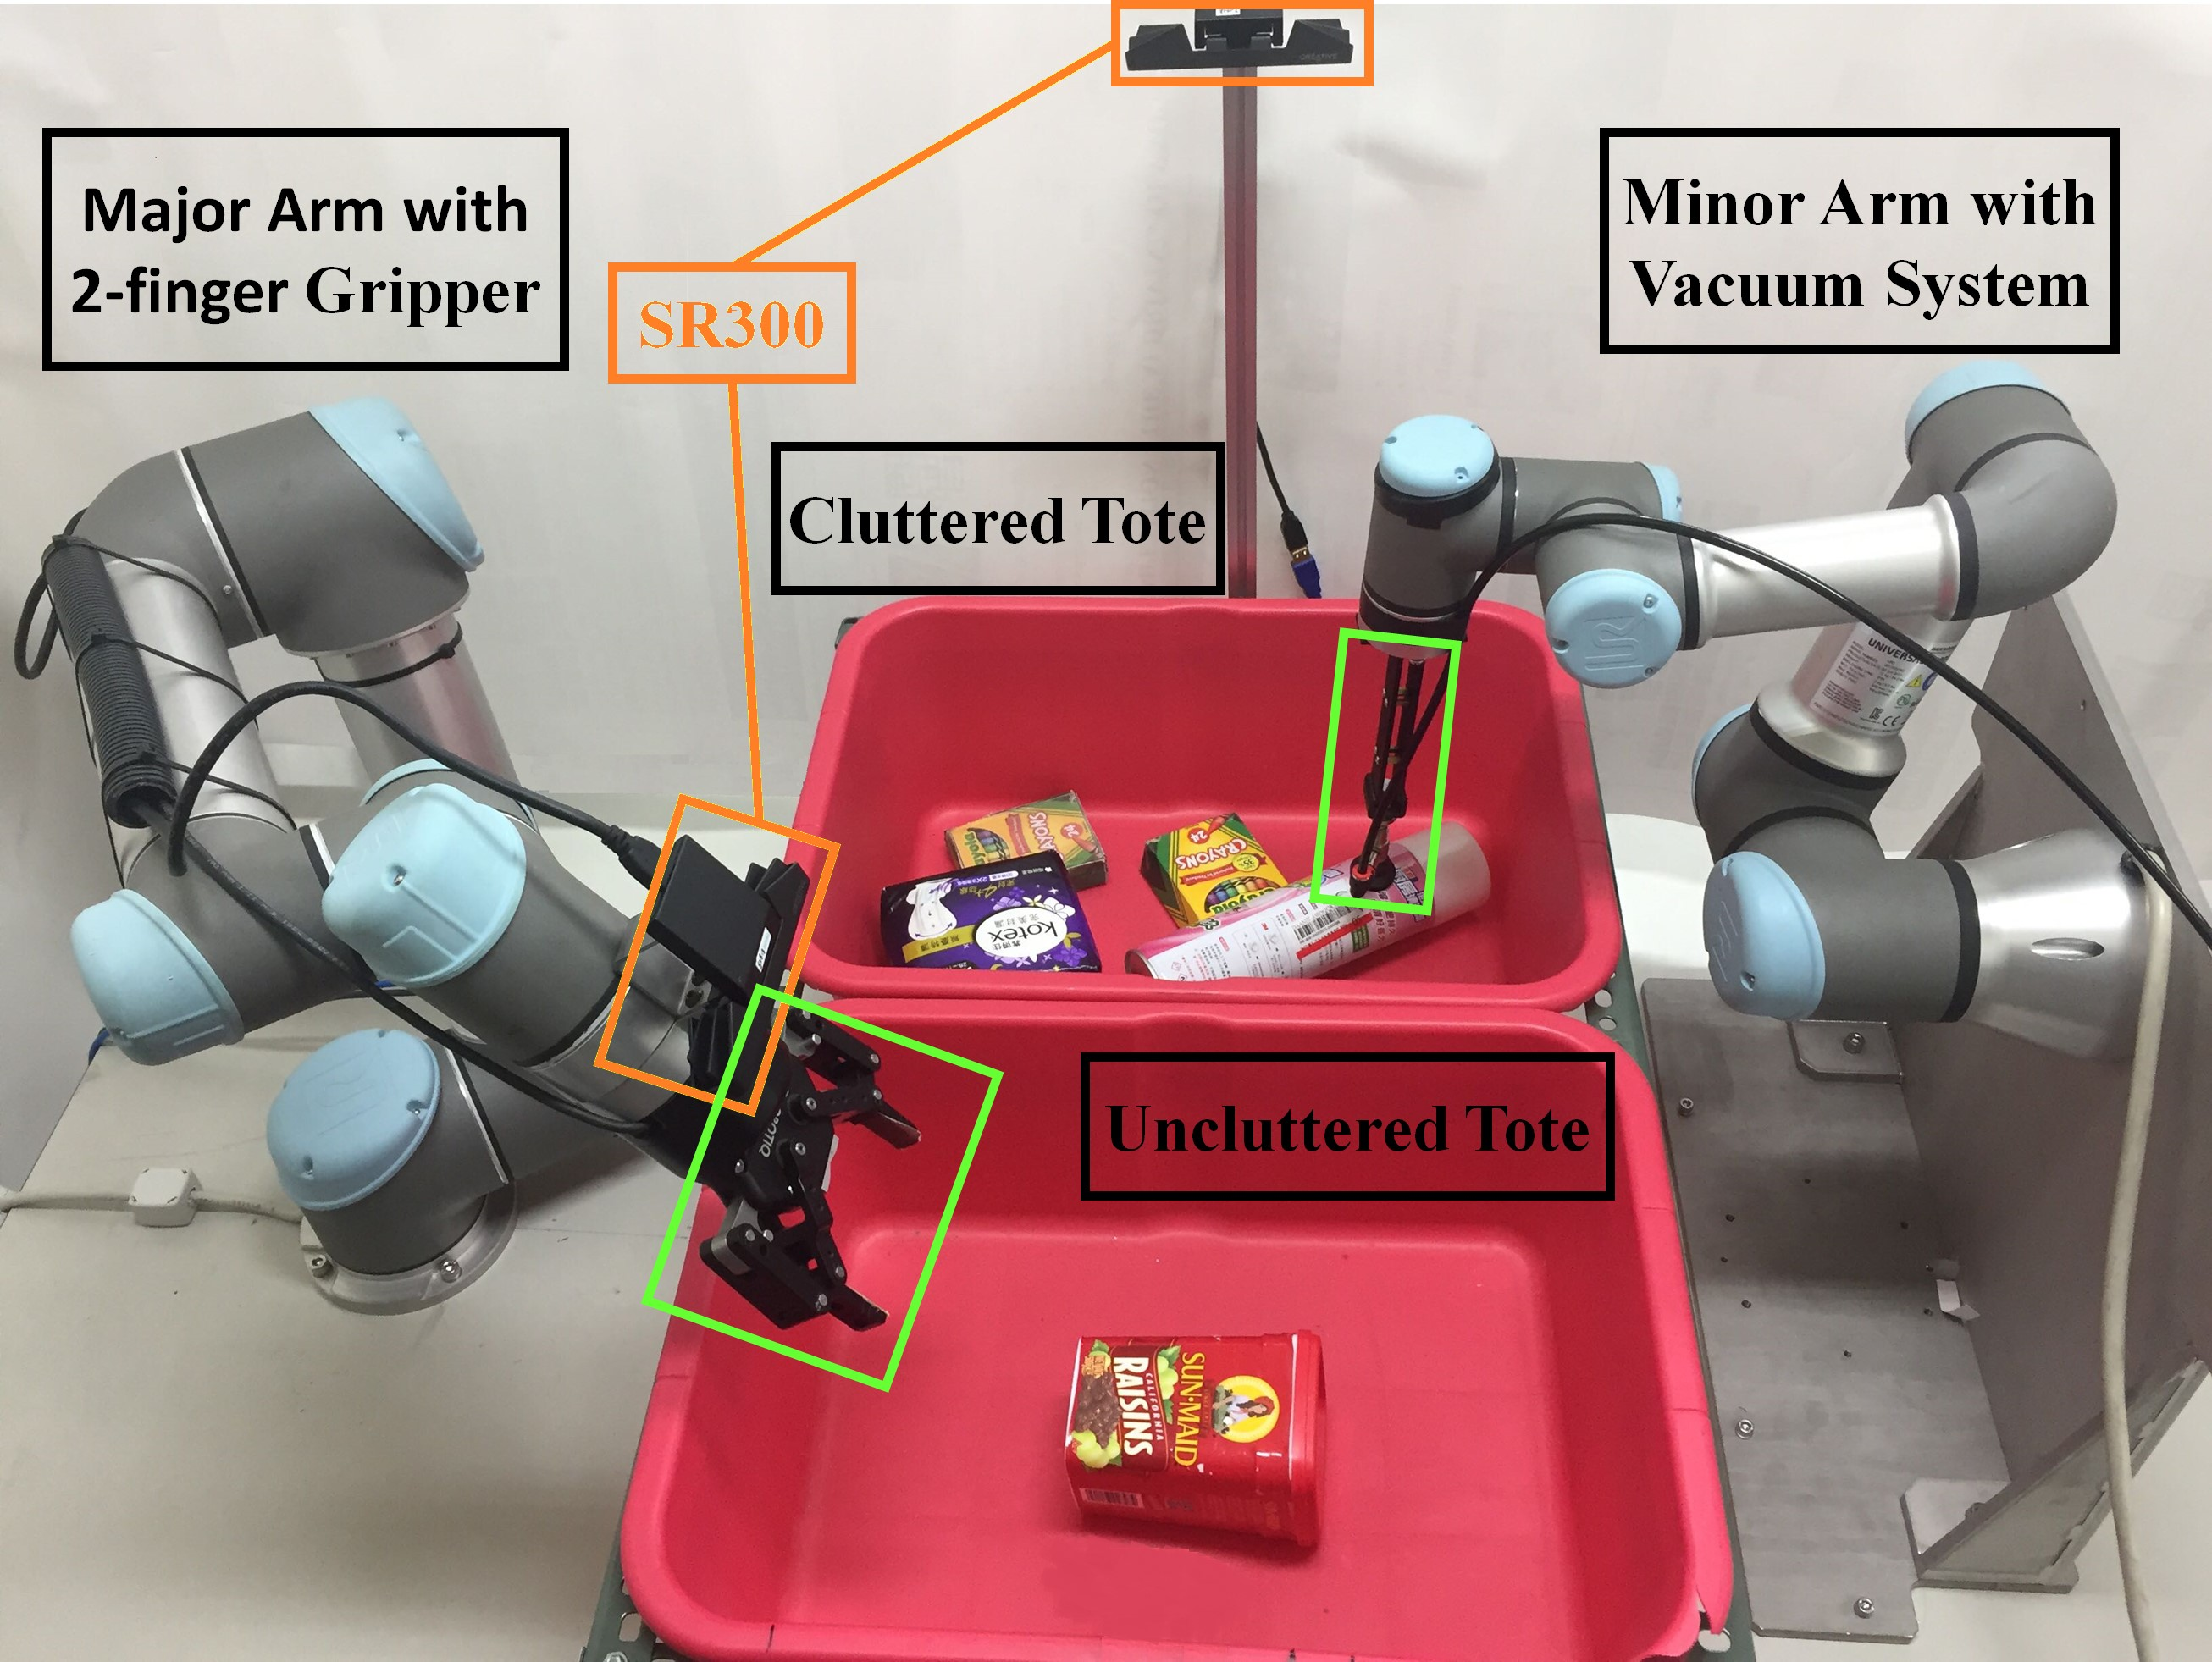
\includegraphics[width=\textwidth]{./figures/robot_system_v2.jpg}
          %\caption{Collaborative robotic arms for pose-aware placing. }
 	\label{fig:robot_system}
      \end{subfigure}
     \begin{subfigure}[t] {0.53\textwidth}
          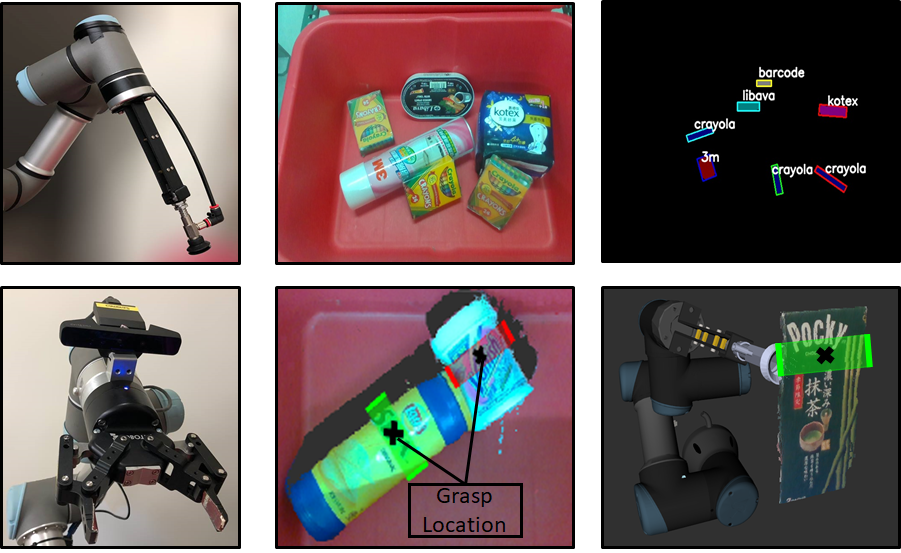
\includegraphics[width=\textwidth]{./figures/affordance_v3.png}
          %\caption{Brandname-based affordance and grasp predictions. }
	\label{fig:brandname-direction}
      \end{subfigure}
   \caption{圖1.左圖:本研究提出雙手臂主動式操作系統去主動改變場景以達到改善機器人感知環境能力,並最佳化物品夾取可行性系統的效果。吸盤假爪從一個雜亂環境移動物品去取得被隱蔽或部分遮蔽的品牌文字資訊。而雙指假爪則藉由基於品牌文字之線索預測夾取點,以此去完成特定姿態的物品擺放任務。右圖:基於品牌文字,本研究可在雜亂環境中預測品牌文字姿態,並以此針對吸盤假爪與雙指假爪進行物品夾取可能性預測。
}
\label{fig:baseline-active}
\end{figure*}

\subsection{多視角主動式視覺}

\subsection{手臂假爪配置}

\section{商品語意資料庫}

\subsection{真實世界訓練集}

\subsection{虛擬世界訓練集}

\subsection{真實世界測試集}

\section{基於品牌文字之夾取可行性預測}

\subsection{品牌文字語意分割}

\subsection{夾取可行性預測}

\section{主動式操作系統}

\subsection{單手臂操作}
本研究專注於透過設計資料庫並用其資料訓練夾取可行性預測系統,並以此作為線索作為雙手臂主動式操

\subsection{夾取可行性預測}
本研究專注於透過設計資料庫並用其資料訓練夾取可行性預測系統,並以此作為線索作為雙手臂主動式操

%\chapter{Reference}
\label{chapter:ref}

Section~\ref{sec:citation} explains how to include citation.
Section~\ref{sec:quote} explains how to use quote.

\section{Citation}
\label{sec:citation}

We use \textbackslash cite\{\} to cite references.
Besides, we need to use $\sim$ to connect \textbackslash cite\{\} and previous text.

For example (請看 .tex 檔),
\begin{itemize}
\item Yang et al.~\cite{Yang_2016} analyzed the strategy and tactics of Reinhard von Lohengramm blablabla.
\item Yang and Fox divides the history of Free Planets into three eras~\cite{Yang_2017}.
\end{itemize}

Note that, when mentioning authors
\begin{itemize}
\item only 1 author: Yang [citation] ...
\item just 2 authors: Yang and Fox [citation] ...
\item more than 2 authors: Yang et al. [citation] ...
\end{itemize}

\section{Quote}
\label{sec:quote}

\textbf{注意:} 在 latex 中使用單/雙引號時要小心, 左邊的引號打法不同 (請看 .tex 檔):
\begin{itemize}
\item `單引號'
\item ``單引號"
\end{itemize}

%\chapter{Figures and Tables}
\label{chapter:fig}

關於怎麼使用圖和表格, 網路上都可以找到許多介紹. Google it.
(其實是我累了, 不想寫了 XD)

\section{Figures}

這裡介紹如何載入一張圖片, 解釋請看 .tex 檔的註解吧!
此外, 我個人習慣是把所有的圖檔都放在一個資料夾下, 像是 \textit{figures/}

\begin{figure}[b]
  \centering
  % 圖片的高度與寬度, height 設為 ! 代表由寬度大小等比例縮放
  \includegraphics[height=!,width=0.4\linewidth,keepaspectratio=true]%
  % 圖片的位置
  {figures/nctu_logo}
  % [] 放的是顯示在 list of figure 的文字
  % {} 放的是顯示在圖下方的文字
  \caption[NCTU logo]{{\footnotesize The history of NCTU days back to 1896 ...}}
  \label{fig:nctu_logo}
\end{figure}

\textbf{注意:} 在呼叫圖的標籤的時候, 請寫 \textbf{Figure$\sim$\textbackslash ref\{label\}}.
(請參考 .tex 檔看我是如何載入 Figure~\ref{fig:nctu_logo} 的吧).

\section{Tables}

我個人的習慣是把表格的內容放到另一個 .tex 內, 再把這些 .tex 檔放到另一個資料夾下 (e.g. \textit{tables/}), 讓本文看起來不會那麼亂.
請參考 Table~\ref{table:clsoptions} 裡面的註解 (檔案位置 \textit{tables/table-classopt.tex}), 看看要怎寫一個簡單的 table 吧.


%-------------------------------------------------------------------------------
% 參考文獻
%-------------------------------------------------------------------------------

% Set bib style
\bibliographystyle{IEEEtran}

% Add Bibliography to "Table of Contents"
\addBibToContents

% Usage:
%   \bibliography{bib/bib1,bib/bib2,...,bib/bibN} % 注意: 不要有空格
%
% For IEEEtran users:
%   DO NOT remove bib/BSTcontrol.bib when using IEEEtran.bst. The reason is that
% when we cite two papers of the same (or similar) authors, IEEEtran.bst would
% replace the author names with "------". To avoid this, we use BSTControl.bib
% to set ctldash_repeated_names to 'no'.
%
% For non IEEEtran users:
%   Please delete bib/ieeeBSTcontrol from \bibliography{}
\bibliography{bib/ieeeBSTcontrol,bib/thesis}
%-------------------------------------------------------------------------------
% 附錄
%-------------------------------------------------------------------------------

% Start appendix
%\appendix

% Add appendicies to "Table of Contents"
\addAppxToContents

% 請從此開始依序擺放附錄
%\chapter{附錄標題}



%-------------------------------------------------------------------------------
% 作者簡歷
%-------------------------------------------------------------------------------

% 簡歷 (Only shown in a PhD dissertation)
%\chapter*{Curriculum Vitae}
\addcontentsline{toc}{chapter}{Curriculum Vitae}
{\bf Wen-Li Yang} is a character in Tanaka Yoshiki's science fiction, ``Die Legende der Sternhelden." His research interests include drinking and sleep.

% 著作列表 (Only shown in a PhD dissertation)
%\begin{publications}%

%%%%%%%%%%%%%%%%%%%%%%%%%%%%%%%%%%%%%%%%%%%%%%%%%%%%%%%%%%%%%%%%%%%%%%%%%%%%%%%

\section*{Journal Papers}
\begin{spacing}{1}
\begin{enumerate}

\item {\bf \underline{Wen-Li Yang}}, Bamboo Fox, ``Carry the Free Planets Star Fleet in Three Ways," \textit{Journal of Galaxy}, vol. 9527, no. 1, pp. 22--66, 2016

\end{enumerate}
\end{spacing}

%%%%%%%%%%%%%%%%%%%%%%%%%%%%%%%%%%%%%%%%%%%%%%%%%%%%%%%%%%%%%%%%%%%%%%%%%%%%%%%

\section*{Conference Papers}
\begin{spacing}{1}
\begin{enumerate}

\item {\bf \underline{楊威利}}, 竹狐, ``如何屌打金髮小子," in \textit{International Conference of Military History}, 2016, Iserlohn, Germany

\end{enumerate}
\end{spacing}

%%%%%%%%%%%%%%%%%%%%%%%%%%%%%%%%%%%%%%%%%%%%%%%%%%%%%%%%%%%%%%%%%%%%%%%%%%%%%%%

\end{publications}

\end{document}
